\documentclass[12pt]{article}
% Load packages
\usepackage{url}  % Formatting web addresses  
\usepackage{ifthen}  % Conditional 
\usepackage{multicol}   %Columns
\usepackage[utf8]{inputenc} %unicode support
\usepackage{amsmath}
\usepackage{amssymb}
\usepackage{epsfig}
\usepackage{epstopdf}
\usepackage{graphicx}
\usepackage[margin=0.1pt,font=footnotesize,labelfont=bf]{caption}
\usepackage{setspace}
%\usepackage{longtable}
\usepackage{colortbl}
%\usepackage{palatino,lettrine}
%\usepackage{times}
%\usepackage[applemac]{inputenc} %applemac support if unicode package fails
%\usepackage[latin1]{inputenc} %UNIX support if unicode package fails
\usepackage[wide]{sidecap}
%\usepackage[authoryear,round,comma,sort&compress]{natbib}
\usepackage[square,sort,comma,numbers]{natbib}
%\usepackage[authoryear,round]{natbib}
\usepackage{supertabular}
\usepackage{simplemargins}
\usepackage{comment}
\usepackage{lineno}

\urlstyle{rm}

%\textwidth = 6.50 in
%\textheight = 9.5 in
%\oddsidemargin =  0.0 in
%\evensidemargin = 0.0 in
%\topmargin = -0.50 in
%\headheight = 0.0 in
%\headsep = 0.25 in
%\parskip = 0.15in
%\linespread{1.75}
\doublespace

%\usepackage{geometry}
\usepackage{fullpage}

%\bibliographystyle{plain}
\bibliographystyle{msb}

\makeatletter
\renewcommand\subsection{\@startsection
	{subsection}{2}{0mm}
	{-0.05in}
	{-0.5\baselineskip}
	{\normalfont\normalsize\bfseries}}
\renewcommand\subsubsection{\@startsection
	{subsubsection}{2}{0mm}
	{-0.05in}
	{-0.5\baselineskip}
	{\normalfont\normalsize\itshape}}
\renewcommand\section{\@startsection
	{subsection}{2}{0mm}
	{-0.2in}
	{0.05\baselineskip}
	{\normalfont\large\bfseries}}	
\renewcommand\paragraph{\@startsection
	{paragraph}{2}{0mm}
	{-0.05in}
	{-0.5\baselineskip}
	{\normalfont\normalsize\itshape}}
\makeatother

%Review style settings
%\newenvironment{bmcformat}{\begin{raggedright}\baselineskip20pt\sloppy\setboolean{publ}{false}}{\end{raggedright}\baselineskip20pt\sloppy}

%Publication style settings

% Single space'd bib -
\setlength\bibsep{0pt}

\renewcommand{\rmdefault}{phv}\renewcommand{\sfdefault}{phv}

% Change the number format in the ref list -
\renewcommand{\bibnumfmt}[1]{#1.}

% Change Figure to Fig.
\renewcommand{\figurename}{Fig.}

% Begin ...
\begin{document}
\begin{titlepage}
{\par\centering\textbf{\Large Dynamic Modeling of Cell Free Metabolic Networks using Effective Kinetic Models}}
\vspace{0.05in}
{\par \centering \large{ Joseph A. Wayman and Jeffrey D. Varner$^{*}$}}
\vspace{0.10in}
{\par \centering \large{School of Chemical and Biomolecular Engineering}}
{\par \centering \large{Cornell University, Ithaca NY 14853}}
\vspace{0.1in}
{\par \centering \textbf{Running Title:}~Modeling cell free metabolism}
\vspace{0.1in}
{\par \centering \textbf{To be submitted:}~\emph{Processes}}
\vspace{0.5in}
{\par \centering $^{*}$Corresponding author:}
{\par \centering Jeffrey D. Varner,}
{\par \centering Associate Professor, School of Chemical and Biomolecular Engineering,}
{\par \centering 244 Olin Hall, Cornell University, Ithaca NY, 14853} 
{\par \centering Email: jdv27@cornell.edu} 
{\par \centering Phone: (607) 255 - 4258}
{\par \centering Fax: (607) 255 - 9166}
\end{titlepage}
\date{}
\thispagestyle{empty}
\pagebreak
%%%%%%%%%%%%%%%%%%%%%%%%%%%%%%%%%%%%%%%%%%%%%%%%%%%%%%%%%%%%%%%%%%%%%%%%%%%%%%%%%%%%%%%%%%%%%%%%%%%%%%%%%%%
%%%%%%%%%%%%%%%%%%%%%%%%%%%%%%%%%%%%%%%%%%%%%%%%%%%%%%%%%%%%%%%%%%%%%%%%%%%%%%%%%%%%%%%%%%%%%%%%%%%%%%%%%%%
\section*{Abstract}

{\noindent \textbf{Keywords:}~Cell free metabolism, Mathematical modeling}

\pagebreak

\setcounter{page}{1}

\linenumbers

\section*{Introduction}
Whole-cell bacterial processes are widely used in biotechnology to produce an array of products including high-value protein therapeutics.
However, whole-cell processes share the central limitation of requiring cell growth, 
which redirects resources away from product synthesis, and cell walls, which complicate interrogation and control of intracellular metabolic processes.
On the other hand, cell-free metabolic systems offer many advantages over traditional in vivo production methods. 
For example, cell-free systems can direct scarce metabolic resources exclusively towards a single product of interest. 
Moreover, with no cell wall, cell free systems can more easily be interrogated, and substrates of the metabolite processes directly controlled.
Cell free production offers the unique opportunity to study metabolism without the complication of cell growth and gene expression processes.
For modeling, this implies that we need only consider allosteric regulation of enzyme activity when building and testing cell free metabolic models.
Of course, modeling allosteric mechanisms is itself a difficult problem when the model is at a whole genome scale. To address this problem, we have developed a
an approach based upon the constrained fuzzy logic framework of Morris and Lauffenburger [REFHERE].

In this study, we present an effective cell free metabolic modeling framework, and test this framework using two proof of concept metabolic models. 
[FINISH].

\clearpage

\section*{Results}
We developed two proof of concept metabolic networks to investigate the features of our effective cell free modeling approach (Fig. \ref{fig-networks}).
In both examples, substrate $S$ was converted to the end-products $P_{1}$ and $P_{2}$ through a series of enzymatically catalyzed reactions, 
including a branch point at hypothetical metabolite $M_{2}$. 
Several of these reactions involved cofactor dependence ($AH$ or $A$), and various allosteric regulation mechanisms. 
Network A included feedback inhibition of the initial pathway enzyme ($E_{1}$) by pathway end products $P_{1}$ and $P_{2}$ (Fig. \ref{fig-networks}A).
On the other hand, network B involved feedback inhibition of $E_{1}$ by $P_{2}$ and $E_{6}$ by $P_{1}$ (Fig. \ref{fig-networks}B). 
In both networks, branch point enzymes $E_{3}$ and $E_{6}$ were subject to feed-forward activation by cofactor $AH$.
Lastly, in both cases pathway enzyme activity was assumed to decay according to a first-order rate law. 
Allosteric regulation of enzyme activity was represented using a novel rule-based strategy, similar in spirit to the 
Constrained Fuzzy Logic (cFL) approach of Lauffenberger and coworkers [REFHERE]. 
In this formulation, Hill-like transfer functions were used to calculate the influence of metabolite abundance upon target enzyme activity. 
When an enzyme was potentially sensitive to more than one regulatory influence, logical rules were used to select which transfer function regulated enzyme 
activity at any given time (Fig. \ref{fig-control-schematic}).      
Thus, our test networks involved important features such as cofactor recycling, enzyme activity and metabolite dynamics, 
as well as multiple overlapping allosteric regulatory mechanisms.  
As such, developing our effective modeling approach using these problems gave us valuable insight into how to develop larger network models, 
without the complication of network size. 

The rule based regulatory strategy captured classic patterns of allosteric activation and inhibition of enzyme activity (Fig. \ref{fig-kinetics-simulations}).  
The first case we explored was substrate activation of enzyme activity (positive cooperativity). 
Classically, we expected a sigmoidal relationship substrate abundance and reaction rate for positive cooperativity. 


End product yield was controlled by feedback inhibition, while selectivity was controlled by branch point enzyme inhibition (Fig. \ref{fig-onoff-simulations}).
A critical test of our modeling approach was to simulate networks with known behavior. If we cannot reproduce the expected behavior of simple networks, then our
modeling strategy, and particularly the rule-based approximation of allosteric regulation, will not be feasible for large scale problems.
We considered two cases,  control on/off, for each network configuration. 
Each of these cases had identical kinetic parameters and initial conditions; 
the \textit{only} differences between the cases was the allosteric regulation rules, and the control parameters associated with these rules. 
As expected, end product accumulation was larger for network A when the control was off (no feedback inhibition of $E_{1}$ by $P_{1}$ and $P_{2}$),
as compared to the on case (Fig. \ref{fig-onoff-simulations}A). We found this behavior was robust to the choice of underlying kinetic parameters, 
as we observed that same qualitative response across an ensemble of randomized parameter sets (N = 100). 
The control on/off response of network B was more subtle. In the off case, the behavior was qualitatively similar to network A. 
However, for the on case, flux was diverted away from $P_{2}$ formation by feedback inhibition of $E_{6}$ activity at the $M_{2}$ branch point by $P_{1}$ (Fig. \ref{fig-onoff-simulations}B).
Lower $E_{6}$ activity at the $M_{2}$ branch point allowed more flux toward $P_{1}$ formation, hence the yield of $P_{1}$ also increased (Fig. \ref{fig-onoff-simulations}C).
Again, the control on/off behavior was robust to the values of the kinetic parameters, as the same qualitative trend was conserved across 
an ensemble of possible randomized kinetic parameters (N = 100). Taken together, these simulations suggested that the rule based allosteric control 
concept could robustly capture expected feedback behavior.

The estimation of kinetic parameters was sensitive to the choice of control structure (Fig. \ref{fig-parameter-fit}).
A critical challenge for any dynamic model effort is the estimation of kinetic parameters. 
However, beyond this challenge is the identification of model structure, i.e., the biological connectivity of the system you are exploring.
Of course these two issues are not independent as any description of the control of enzyme activity will be a function of the system state, which
in turn is a function of the kinetic parameters.

Discrimination between competing model formulations can be achieved by optimal experimental design (Fig. ZZ). [FINISH]



\clearpage

\section*{Discussion}
In this study, we proposed a dynamic modeling strategy to simulate cell free metabolic networks. We demonstrated this strategy using two proof of concept metabolic networks 
with the same enzymatic connectivity, but differing control structures. [FINISH]

Cybernetic models, other dynamic models of metabolism. 

While the results of this study were encouraging, there are several critical next steps that must be accomplished before we can model genome scale cell free metabolic networks.
[FINISH]

\section*{Materials and Methods}

\subsection*{Formulation and solution of the model equations.}
We used ordinary differential equations (ODEs) to model the time evolution of metabolite ($x_{i}$) and scaled enzyme ($\epsilon_{i}$) abundance in hypothetical cell free
metabolic networks:
\begin{eqnarray}
	\frac{dx_{i}}{dt} & = & \sum_{j = 1}^{\mathcal{R}}\sigma_{ij}r_{j}\left(\mathbf{x},\mathbf{\epsilon},\mathbf{k}\right)\qquad{i=1,2,\hdots,\mathcal{M}}\\
	\frac{d\epsilon_{i}}{dt} & = & -\lambda_{i}\epsilon_{i}\qquad{i = 1,2,\hdots,\mathcal{E}}
\end{eqnarray}where $\mathcal{R}$ denotes the number of reactions, $\mathcal{M}$ denotes the number of metabolites and $\mathcal{E}$ denotes the number of
enzymes in the model. The quantity $r_{j}\left(\mathbf{x},\mathbf{\epsilon},\mathbf{k}\right)$ 
denotes the rate of reaction $j$. Typically, reaction $j$ is a non-linear function of metabolite and enzyme abundance, as well as unknown kinetic parameters 
$\mathbf{k}$ ($\mathcal{K}\times{1}$).
The quantity $\sigma_{ij}$ denotes the stoichiometric coefficient for species $i$ in reaction $j$. If 
$\sigma_{ij}>0$, metabolite $i$ is produced by reaction $j$. Conversely, if $\sigma_{ij}>0$, metabolite $i$ is consumed by reaction $j$, while $\sigma_{ij} = 0$ indicates
metabolite $i$ is not connected with reaction $j$. 
Each reaction rate was written as the product of a reaction term ($\bar{r}_{j}$) and a regulatory term ($v_{j}$):
\begin{equation}
	r_{j}\left(\mathbf{x},\mathbf{\epsilon},\mathbf{k}\right) = \bar{r}_{j}v_{j}
\end{equation}We used multiple saturation kinetics to model the reaction term $\bar{r}_{j}$:
\begin{equation}\label{eqn:rate-bar}
	\bar{r}_{j} = k_{j}^{max}\epsilon_{i}\left(\prod_{s\in{m_{j}^{-}}}\frac{x_{s}}{K_{js} + x_{s}}\right)
\end{equation}where $k_{j}^{max}$ denotes the maximum rate for reaction $j$, $\epsilon_{i}$ denotes the scaled enzyme activity which catalyzes reaction $j$, and
$K_{js}$ denotes the saturation constant for species $s$ in reaction $j$. 
The product in Eqn. \eqref{eqn:rate-bar} was carried out over the set of \textit{reactants} for reaction $j$ (denoted as $m_{j}^{-}$). 
The allosteric regulation term $v_{j}$ depended upon the combination of factors which influenced the activity of enzyme $i$.
For each enzyme, we used a rule based approach to select from competing control factors (Fig. \ref{fig-control-schematic}). 
If an enzyme was activated by $m$ metabolites, we modeled this activation as:
\begin{equation}
	v_{j} = \max\left(f_{1j}\left(x\right),\hdots,f_{mj}\left(x\right)\right)
\end{equation}Conversely, if enzyme activity was inhibited by a $m$ metabolites, we modeling this inhibition as:
\begin{equation}
	v_{j} = 1 - \max\left(f_{1j}\left(x\right),\hdots,f_{mj}\left(x\right)\right)
\end{equation}Lastly, if an enzyme had both $m$ activating and $n$ inhibitory factors, we modeled the regulatory term as:
\begin{equation}
	v_{j} = \min\left(u_{j},d_{j}\right)
\end{equation}where:
\begin{eqnarray}
	u_{j} &=& \max_{j^{+}}\left(f_{1j}\left(x\right),\hdots,f_{mj}\left(x\right)\right) \\
	d_{j} &=& 1 - \max_{j^{-}}\left(f_{1j}\left(x\right),\hdots,f_{nj}\left(x\right)\right)
\end{eqnarray}where $j^{+}$ and $j^{-}$ denote the sets of activating, and inhibitory factors for enzyme $j$. 
If an enzyme had no allosteric factors, we set $v_{j} = 1$.
In this study, each individual factor had the form:
\begin{equation}
	f_{i}\left(\mathbf{x}\right) = \frac{\kappa_{ij}^{\eta}x_{j}^{\eta}}{1 + \kappa_{ij}^{\eta}x_{j}^{\eta}}
\end{equation}where $x_{j}$ denotes the abundance of metabolite $j$, and $\kappa_{ij}$ and $\eta$ are control parameters. 
The model equations were encoded using the Octave programming language, and solved using the LSODE routine in Octave [REFHERE].

\subsection*{Estimation of model parameters from synthetic experimental data}
Model parameters were estimated by minimizing the difference between simulations and synthetic experimental data using particle swarm optimization [REFHERE].
In this study, the parameter estimation problem took the form:
\begin{equation}\label{eqn:objective-function}
	\min_{\mathbf{k}} \sum_{\tau=1}^{\mathcal{T}}\sum_{j=1}^{\mathcal{S}}\left(\frac{\hat{x}_{j}\left(\tau\right) - x_{j}\left(\tau,\mathbf{k}\right)}{\omega_{j}\left(\tau\right)}\right)^{2}
\end{equation}where $\hat{x}_{j}\left(\tau\right)$ denotes the measured value of species $j$ at time $\tau$, $x_{j}\left(\tau,\mathbf{k}\right)$ denotes the simulated 
value for species $j$ at time $\tau$, and $\omega_{j}\left(\tau\right)$ denotes the experimental measurement variance for species $j$ at time $\tau$. The outer summation is respect to
time, while the inner summation is with respect to state. We wanted to approximate a realistic model identification scenario, thus we assumed noisy experimental data, 
limited sampling resolution (approximately 20 minutes per sample) and that only a subset of metabolites were measurable. 

We minimized Eqn. \eqref{eqn:objective-function} using Particle swarm optimization (PSO).
PSO is global optimization procedure which uses a swarming metaheuristic to explore high-dimensional parameter spaces. 
A strength of PSO is its ability to find the global minimum, even in the presence of potentially many local minima, by communicating the local
error landscape experienced by each particle collectively to the swarm using the update rules:
\begin{eqnarray}
	\mathbf{\Delta}_{i} &=&\theta_{1}\mathbf{\Delta}_{i} + \theta_{2}\mathbf{r}_{1}\left(\mathcal{L}_{i} - \mathbf{k}_{i}\right) + \theta_{3}\mathbf{r}_{2}\left(\mathcal{G} - \mathbf{k}_{i}\right) \\
	\mathbf{k}_{i} &=& \mathbf{k}_{i} + \mathbf{\Delta}_{i}
\end{eqnarray}where $\left(\theta_{1},\theta_{2},\theta_{3}\right) = (1.0,0.05564,0.02886)$ are adjustable parameters, $\mathcal{L}_{i}$ denotes local best solution found by particle $i$, and
$\mathcal{G}$ denotes the best solution found over the entire population of particles. The quantities $r_{1}$ and $r_{2}$ denote uniform random vectors with the same dimension as the number of unknown model
parameters ($\mathcal{K}\times{1}$). The PSO algorithm, and the objective function were encoded and solved in the Octave programming language [REFHERE].

\subsection{Model discrimination}


\section*{Acknowledgements}
This study was supported by the National Science Foundation GK12 award (DGE-1045513) 
and by the National Science Foundation CAREER award (FILLMEIN).

\clearpage
%\bibliographystyle{plain}
%\bibliographystyle{IEEEbib}

\bibliography{References_v1}

%\begin{comment}

\clearpage

\begin{figure}
\centering
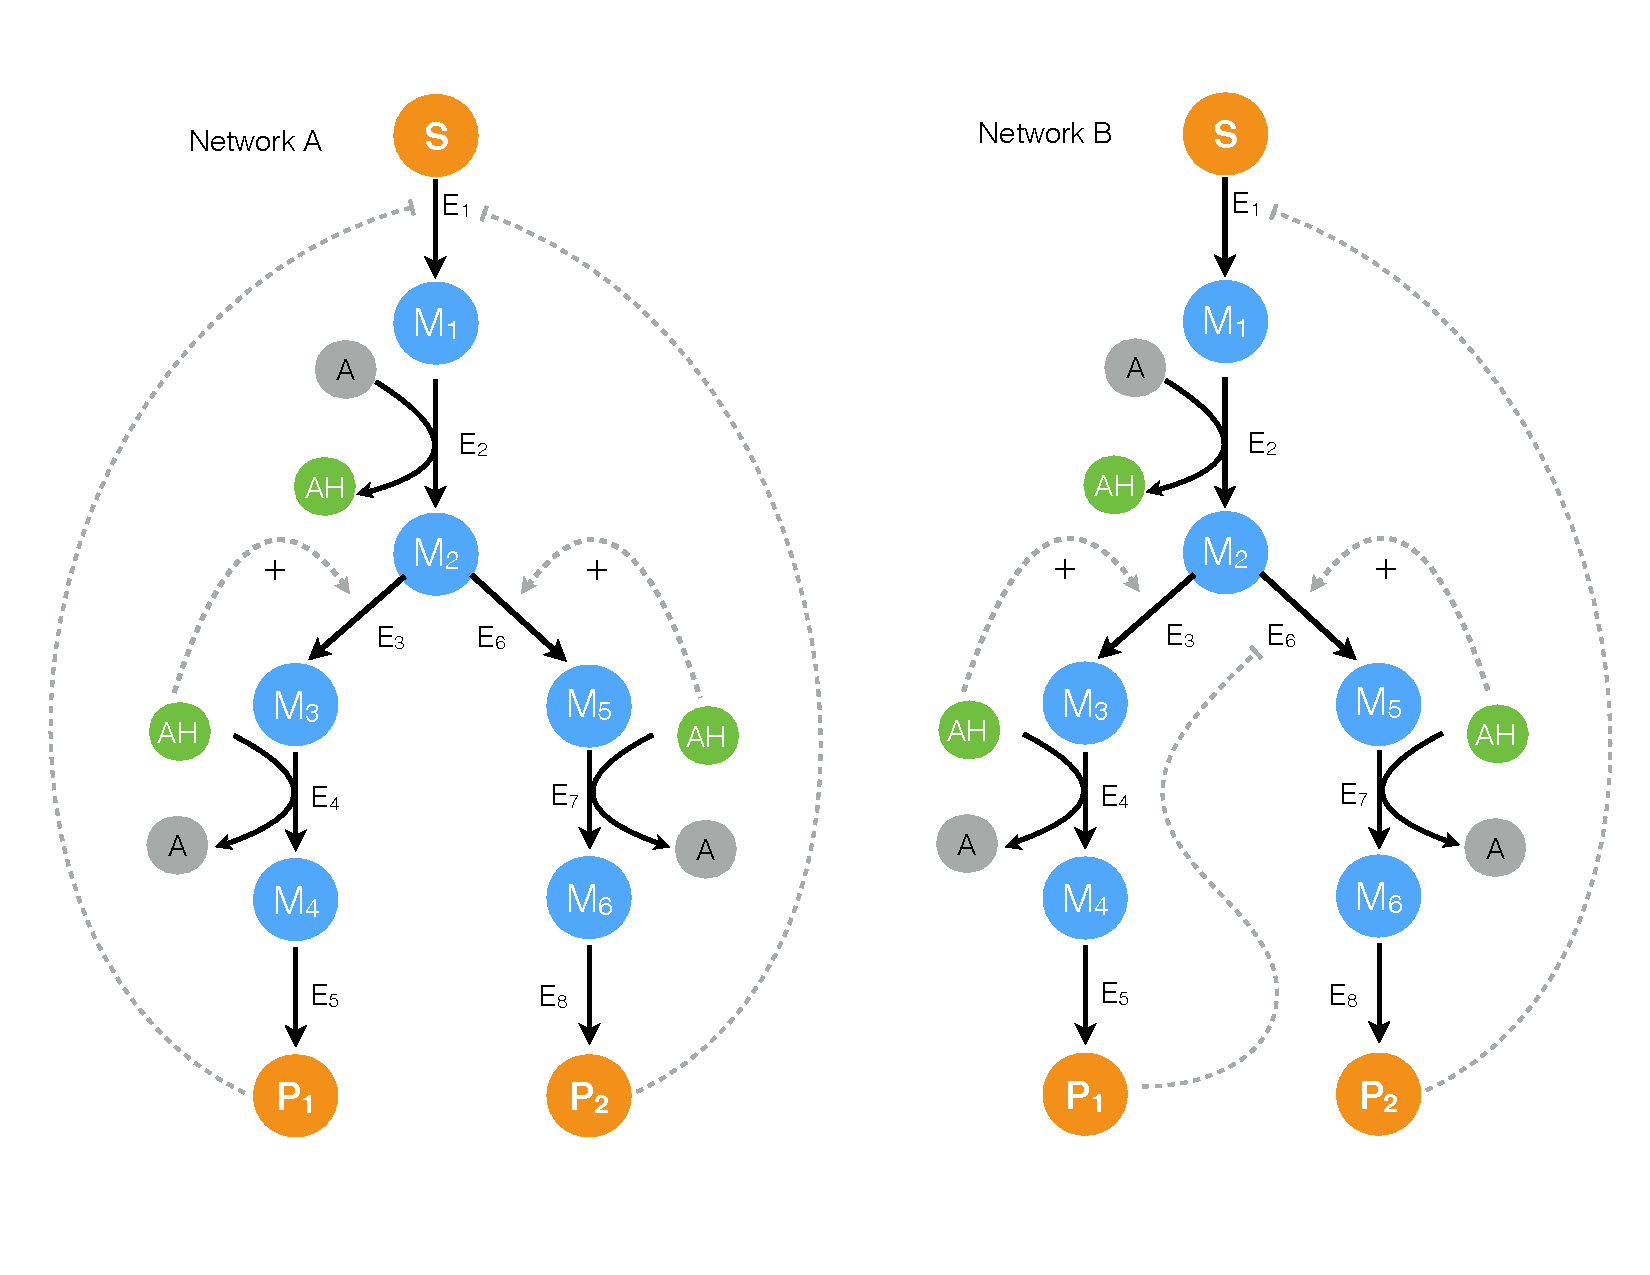
\includegraphics[width=1.0\textwidth]{./figs/Figure-1-Networks.pdf}
\caption{Proof of concept cell-free metabolic networks considered in this study. Substrate $S$ is converted to products $P_{1}$ and $P_{2}$ through a series of chemical conversions
catalyzed by enzyme(s) $E_{j}$. The activity of the pathway enzymes is subject to both positive and negative allosteric regulation. }\label{fig-networks}
\end{figure}

\clearpage

\begin{figure}
\centering
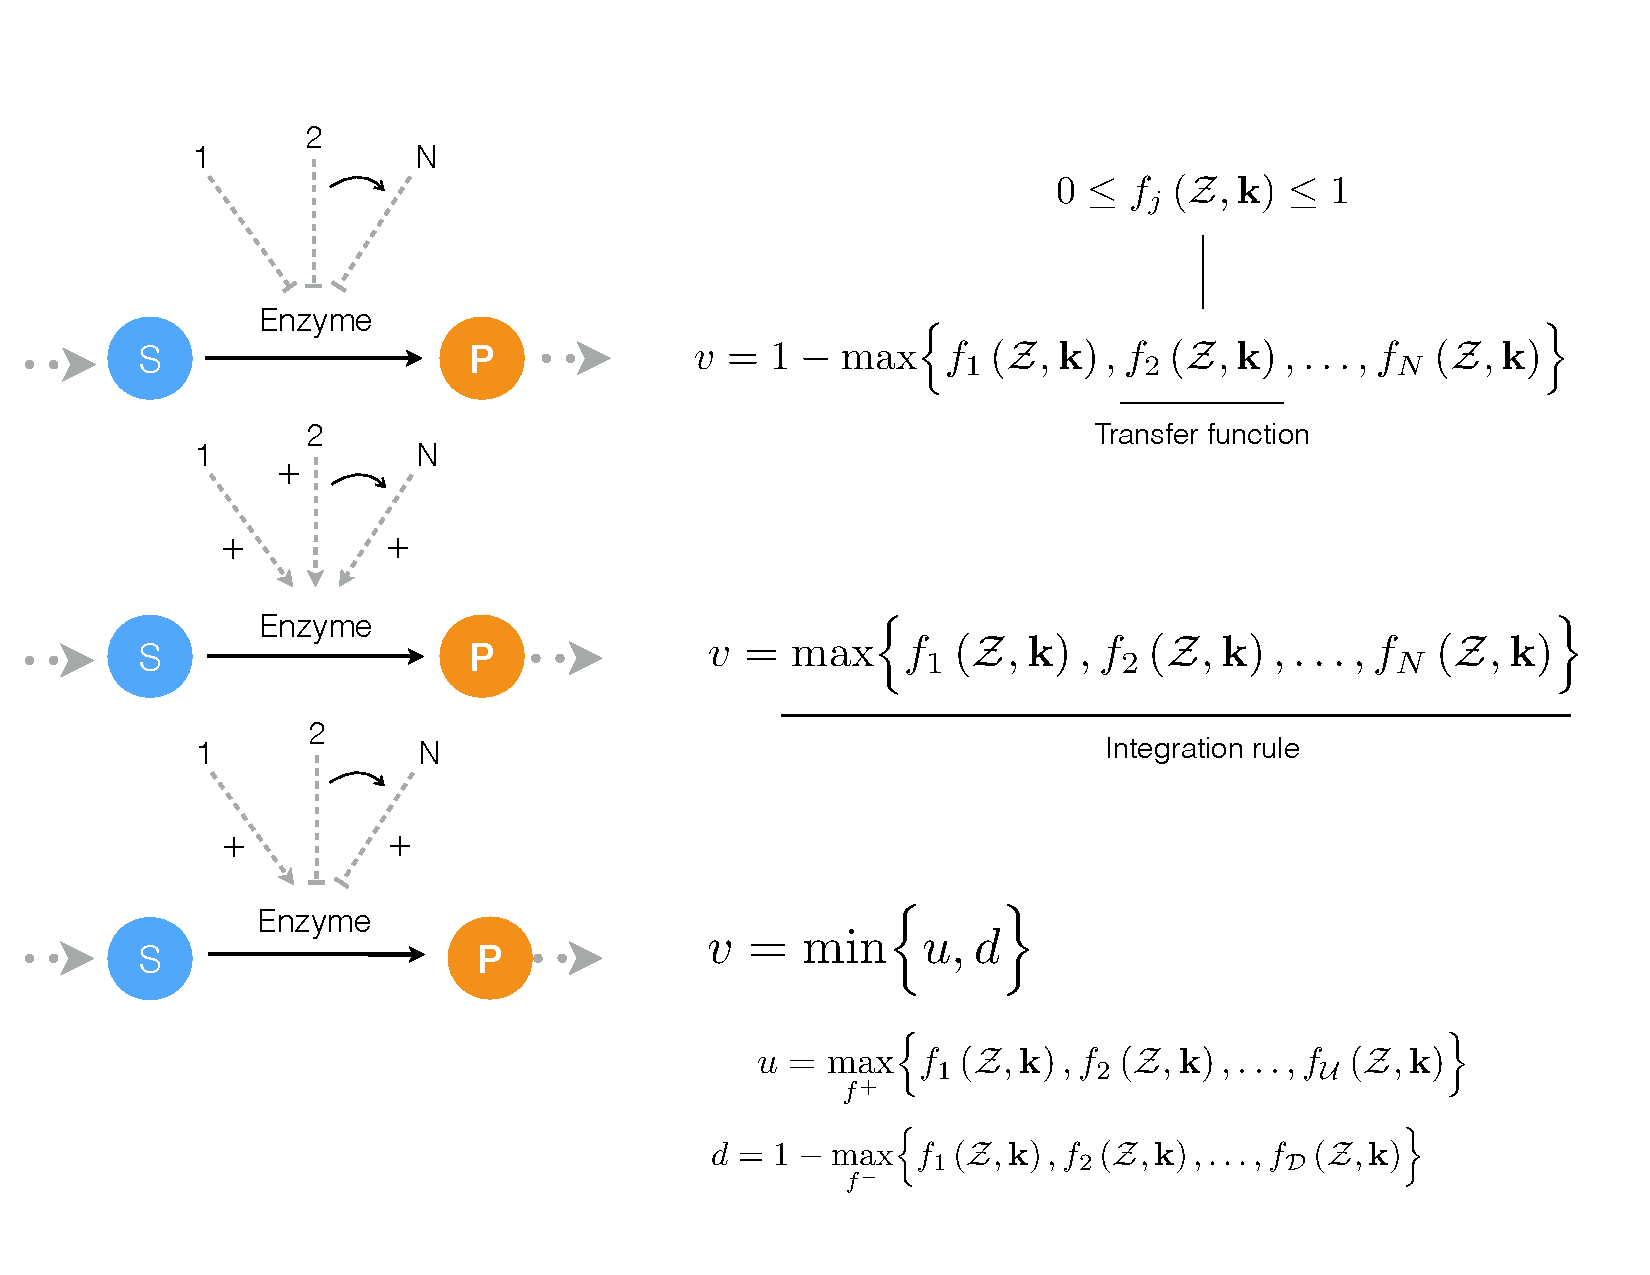
\includegraphics[width=1.0\textwidth]{./figs/Figure-2-ControlSchematic.pdf}
\caption{Schematic of the rule based allosteric enzyme activity control laws. }\label{fig-control-schematic}
\end{figure}

\clearpage

\begin{figure}
\centering
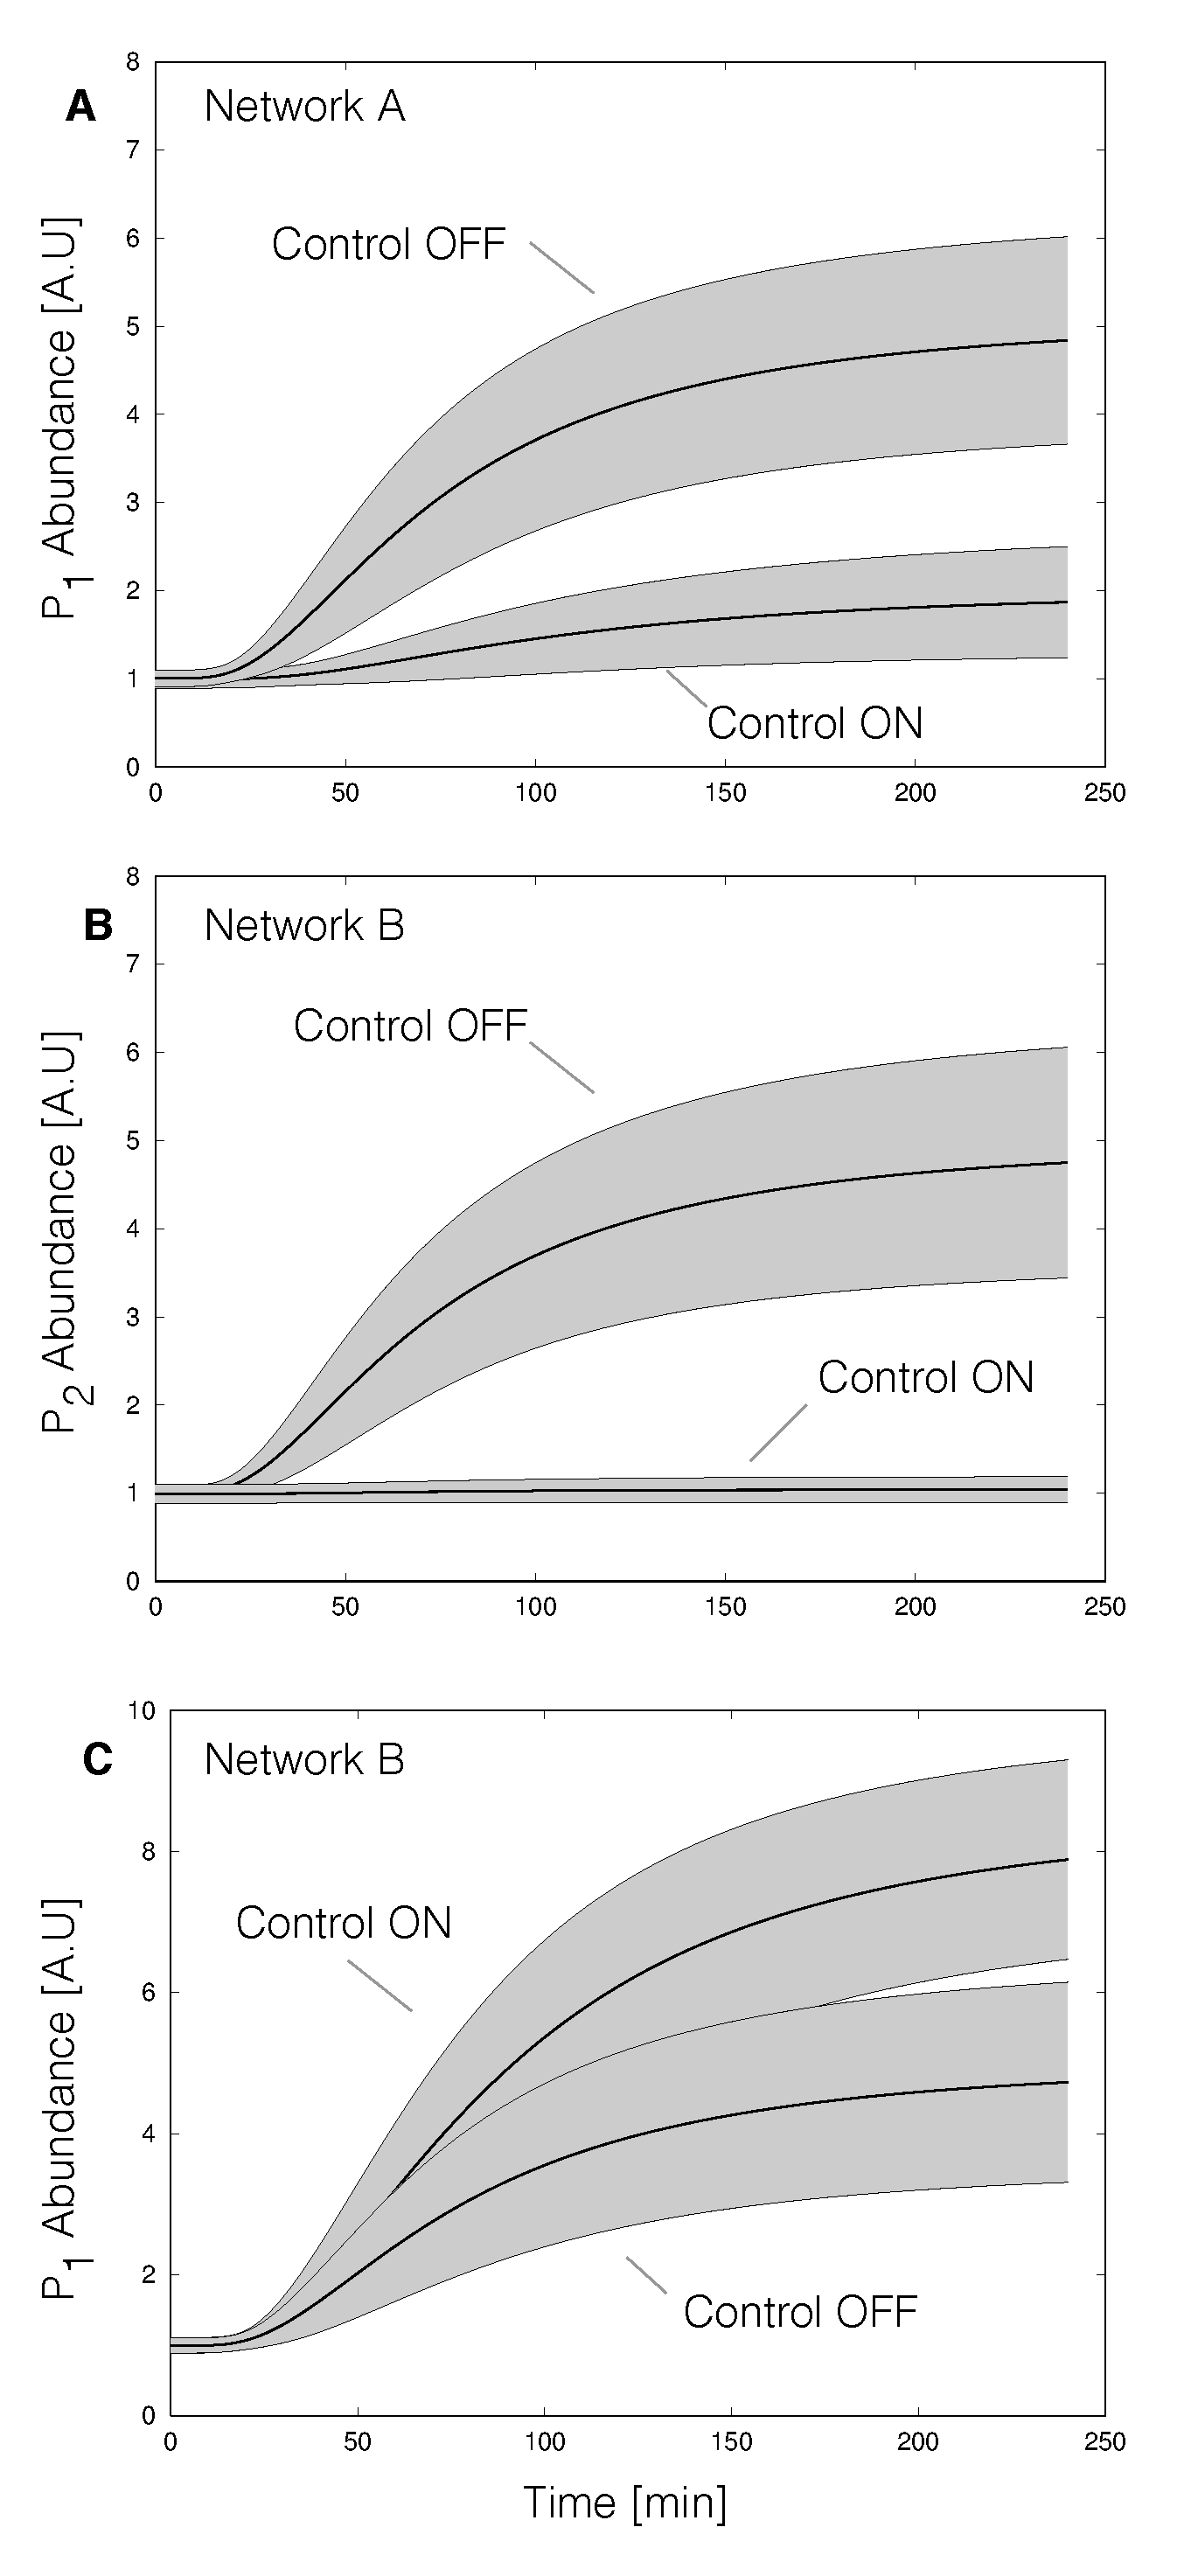
\includegraphics[width=0.55\textwidth]{./figs/Figure-3-OnOffSimulations.pdf}
\caption{On/off control simulations for network A and network B for an ensemble of kinetic parameter sets. 
For each case, N = 100 simulations were conducted using kinetic and initial conditions randomly generated from a hypothetical true parameter set. 
The gray area represents $\pm$ one standard deviation surrounding the mean. Control parameters were fixed during the ensemble calculations.}\label{fig-onoff-simulations}
\end{figure}

\clearpage

\begin{figure}
\centering
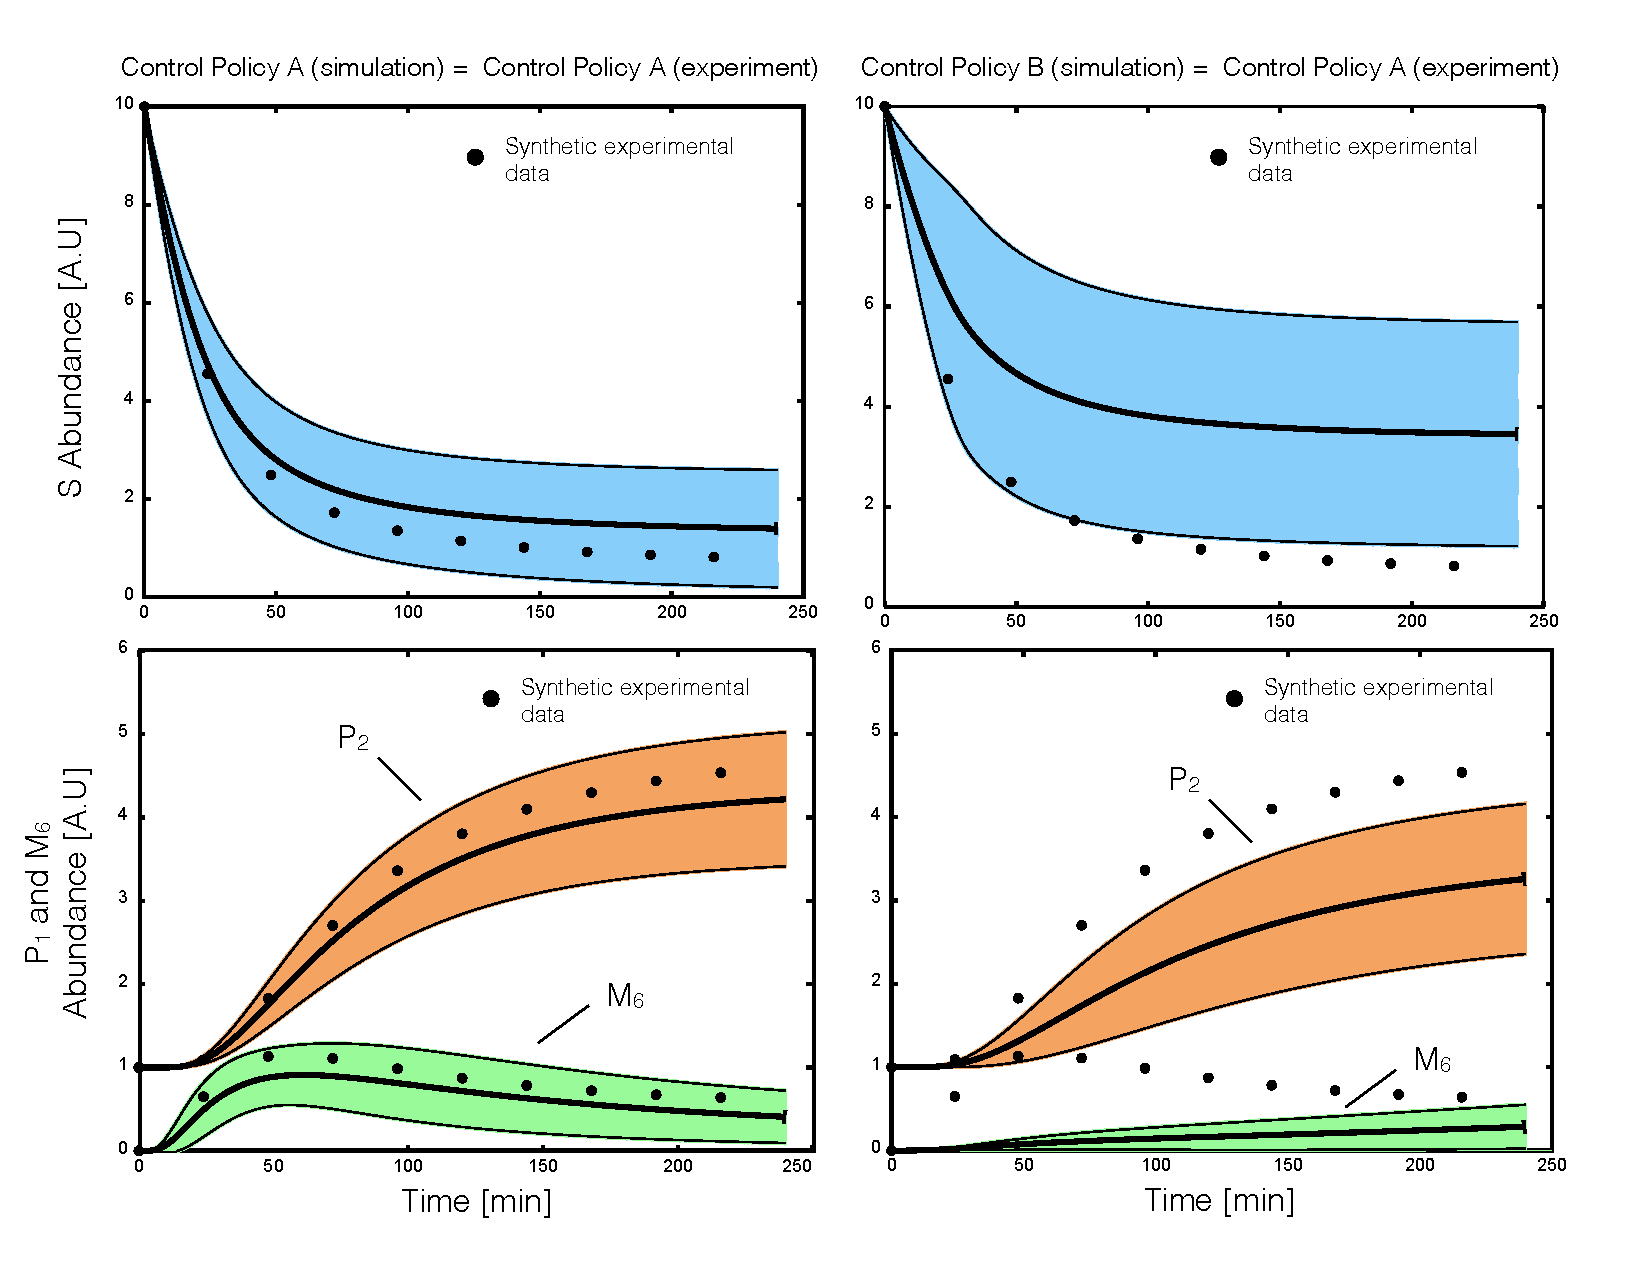
\includegraphics[width=1.0\textwidth]{./figs/Figure-4-ParameterFit.pdf}
\caption{Parameter estimation from synthetic data for the same and mismatched allosteric control logic. }\label{fig-parameter-fit}
\end{figure}

\clearpage

% Supplemental figures -
% Set the S- 
\renewcommand\thefigure{S\arabic{figure}}
\renewcommand\thetable{T\arabic{table}}
\renewcommand\thepage{S-\arabic{page}}
\renewcommand\theequation{S\arabic{equation}}

% Reset the counters -
\setcounter{equation}{0}
\setcounter{table}{0}
\setcounter{figure}{0}
\setcounter{page}{1}

\end{document}

